\documentclass[10 pt,usenames,dvipsnames, oneside]{article}
\usepackage{../../../modelo-ensino-medio}



\begin{document}

\begin{center}
  \begin{minipage}[l]{3cm}

\includegraphics[width=2cm]{logo}    
\end{minipage}\hfill
\begin{minipage}[r]{.8\textwidth}
 {\Large \scshape Atividade: Cálculos com régua}  
\end{minipage}
\end{center}
\vspace{.2cm}

\ifdefined\prof
%Habilidades da BNCC
\begin{objetivos}
\item \textbf{EM13MAT305} Resolver e elaborar problemas com funções logarítmicas nos quais seja necessário compreender e interpretar a variação das grandezas envolvidas, em contextos como os de abalos sísmicos, pH, radioatividade, Matemática Financeira, entre outros.
\end{objetivos}

%Caixa do Para o Professor
\begin{goals}
%Objetivos específicos
\begin{enumerate}
\item Desenvolver operações de multiplicação e divisão utilizando a soma de logaritmos.
\item Efetuar cálculos de multiplicação e divisão utilizando a régua de cálculo.
\end{enumerate}

\tcblower

%Orientações e sugestões
\begin{itemize}
\item Recomenda-se que se destaque um problema na utilização da régua em base dois: os números crescem rápido demais. Aqui seria possível questionar aos alunos como esse problema poderia ser resolvido, antes de apresentar a resposta: tomar uma base menor (mas que ainda precisará ser maior do que $1$, caso contrário teríamos uma escala decrescente na régua).

Recomenda-se então que os estudantes utilizem, em grupos, as réguas disponíveis com o material para efetuar as operações indicadas. O/A professor/a pode tirar cópias das réguas no anexo, recortá-las e entregar aos alunos para que não sejam removidas do material.
\end{itemize}
\end{goals}

\bigskip
\begin{center}
{\large \scshape Atividade}
\end{center}
\fi

Em pequenos grupos, vamos utilizar as réguas de cálculo para efetuar os seguintes cálculos:
\begin{enumerate}
 \begin{multicols}{2}
 \item 9 x 7. %\textcolor{blue}{Basta colocar deslizar a metade superior de modo que o número 1 esteja sobre o número 9 da régua inferior e observar a resposta 63 abaixo do número 7 da metade superior.}
  \item 3,5 x 4.% \textcolor{blue}{Basta colocar deslizar a metade superior de modo que o número 1 esteja sobre o número 3,5 da régua inferior e observar a resposta 14 abaixo do número 4 da metade superior.}
  \item 2,8 x 2,5.% \textcolor{blue}{Basta colocar deslizar a metade superior de modo que o número 1 esteja sobre o número 2,8 da régua inferior e observar a resposta 7 abaixo do número 2,5 da metade superior.}
  \item 28 x 25.% \textcolor{blue}{Apesar dos números 28 e 25 estarem nas duas metades da régua, a posição onde estaria a reposta fica além do comprimento da régua, mas podemos realizar esse cálculo lembrando que $28 \times 25 = 2,8 \times 2,5 \times 10^2 = 7 \times 10^2 = 700$.}
  \item 3,2 x 3,1.% \textcolor{blue}{Ao aplicarmos o procedimento a resposta parece dar $9,9$. Isso ocorre pois há um limite para a escala de graduações escrita na régua, que tem precisão máxima de uma casa decimal para números menores do que 10 e precisão apenas da parte inteira para números maiores do que 10. A resposta exata seria 9,92 e a resposta 9,9 é uma aproximação para ela.}
 \item 5,8 x 9,3.% \textcolor{blue}{A régua mostra a aproximação 54, que está bastante próxima da resposta exata 53,94.}
 \item 583 x 93.% \textcolor{blue}{$583 \times 93 = 5,83 \times 9,3 \times 10^3 \approx 54 \times 10^3 = 54000$, que é uma aproximação para a resposta exata 54219.}
 \item 78326 x 648.% \textcolor{blue}{$78326 \times 648 = 7,8326 \times 6,48 \times 10^6 \approx 51 \times 10^6 = 51000000$, que é uma aproximação para a resposta exata 50755248.}
 \item 56 $\div$ 7.% \textcolor{blue}{Basta colocar deslizar a metade superior de modo que o número 7 esteja sobre o número 56 da régua inferior e observar a resposta 8 abaixo do número 1 da metade superior. Essa operação funciona pois a resposta para $56 \div 7$ é o número que multiplicado por 7 da 56, de modo que, ao colocarmos o número 7 sobre o número 56, o número abaixo do 1 é a resposta para $56 \div 7$.}
 \item 58 $\div$ 4. %\textcolor{blue}{A régua mostra um valor entre 14 e 15, nesses casos podemos tomar a média entre eles, 14,5, que, por acaso, acaba coincidindo com a resposta exata.}
 \item 93 $\div$ 5.% \textcolor{blue}{A régua mostra um valor entre 18 e 19, nesses casos podemos tomar a média entre eles, 18,5, que aproxima resposta exata 18,6.}
 \item 476 $\div$ 93.% \textcolor{blue}{$476 \div 93 = 47,6 \div 9,3 \approx 5,1$, que é uma aproximação para a resposta dada pela calculadora 5,11827957 (que é apenas uma aproximação...).}
 \item 7345 $\div$ 57.% \textcolor{blue}{$7345 \div 57 =73,45 \div 5,7 \times 10\approx 12,5 \times 10 = 125$, que é uma aproximação para a resposta dada pela calculadora 128,859649123 (que é apenas uma aproximação...).}
 \end{multicols}
\end{enumerate}

\ifdefined\prof
\begin{solucao}

Nessas atividades basta deslizar a metade superior de modo que o número 1 esteja sobre o primeiro dos fatores e observar a resposta abaixo do segundo fator na régua superior.

	\begin{enumerate}
	\item $9 \times 7 = 63$.
	\item $3{,}5 \times 4 = 14$.
	\item $2{,}8 \times 2,5 = 7$.
	\item $28 \times 25 = 700$. Apesar dos números $28$ e $25$ estarem nas duas metades da régua, a posição onde estaria a reposta fica além do comprimento da régua, mas podemos realizar esse cálculo lembrando que $28 \times 25 = 2{,}8 \times 2{,}5 \times 10^2 = 7 \times 10^2 = 700$.
	\item $3{,}2 \times 3{,}1 \approx 9{,}9$. Ao aplicarmos o procedimento a resposta parece dar $9,9$. Isso ocorre pois há um limite para a escala de graduações escrita na régua, que tem precisão máxima de uma casa decimal para números menores do que $10$ e precisão apenas da parte inteira para números maiores do que $10$. A resposta exata seria $9{,}92$ e a resposta $9{,}9$ é uma aproximação para ela.
	\item $5{,}8 \times 9{,}3 \approx 54$. A régua mostra a aproximação $54$, que está bastante próxima da resposta exata $53{,}94$.
	\item $583 \times 93\approx 54000$. $583 \times 93 = 5,83 \times 9,3 \times 10^3 \approx 54 \times 10^3 = 54000$, que é uma aproximação para a resposta exata $54219$.
	\item $78326 \times 648 \approx 51000000$. $78326 \times 648 = 7,8326 \times 6,48 \times 10^6 \approx 51 \times 10^6 = 51000000$, que é uma aproximação para a resposta exata $50755248$.
	\item $56 \div 7 = 8$.
	\item $58 \div 4 = 14{,}5$. A régua mostra um valor entre $14$ e $15$, nesses casos podemos tomar a média entre eles, $14{,}5$, que, por acaso, acaba coincidindo com a resposta exata.
	\item $93 \div 5 \approx 18{,}6$. A régua mostra um valor entre $18$ e $19$, nesses casos podemos tomar a média entre eles, $18{,}5$, que aproxima resposta exata $18{,}6$.
	\item $476 \div 93 \approx 5{,}1$. $476 \div 93 = 47{,}6 \div 9{,}3 \approx 5{,}1$, que é uma aproximação para a resposta dada pela calculadora $5{,}11827957$ (que é apenas uma aproximação...).
	\item $7345 \div 57 \approx 125$. $7345 \div 57 =73,45 \div 5{,}7 \times 10\approx 12{,}5 \times 10 = 125$, que é uma aproximação para a resposta dada pela calculadora $128{,}859649123$ (que é apenas uma aproximação...).
\end{enumerate}

\end{solucao}
\fi

\begin{center}
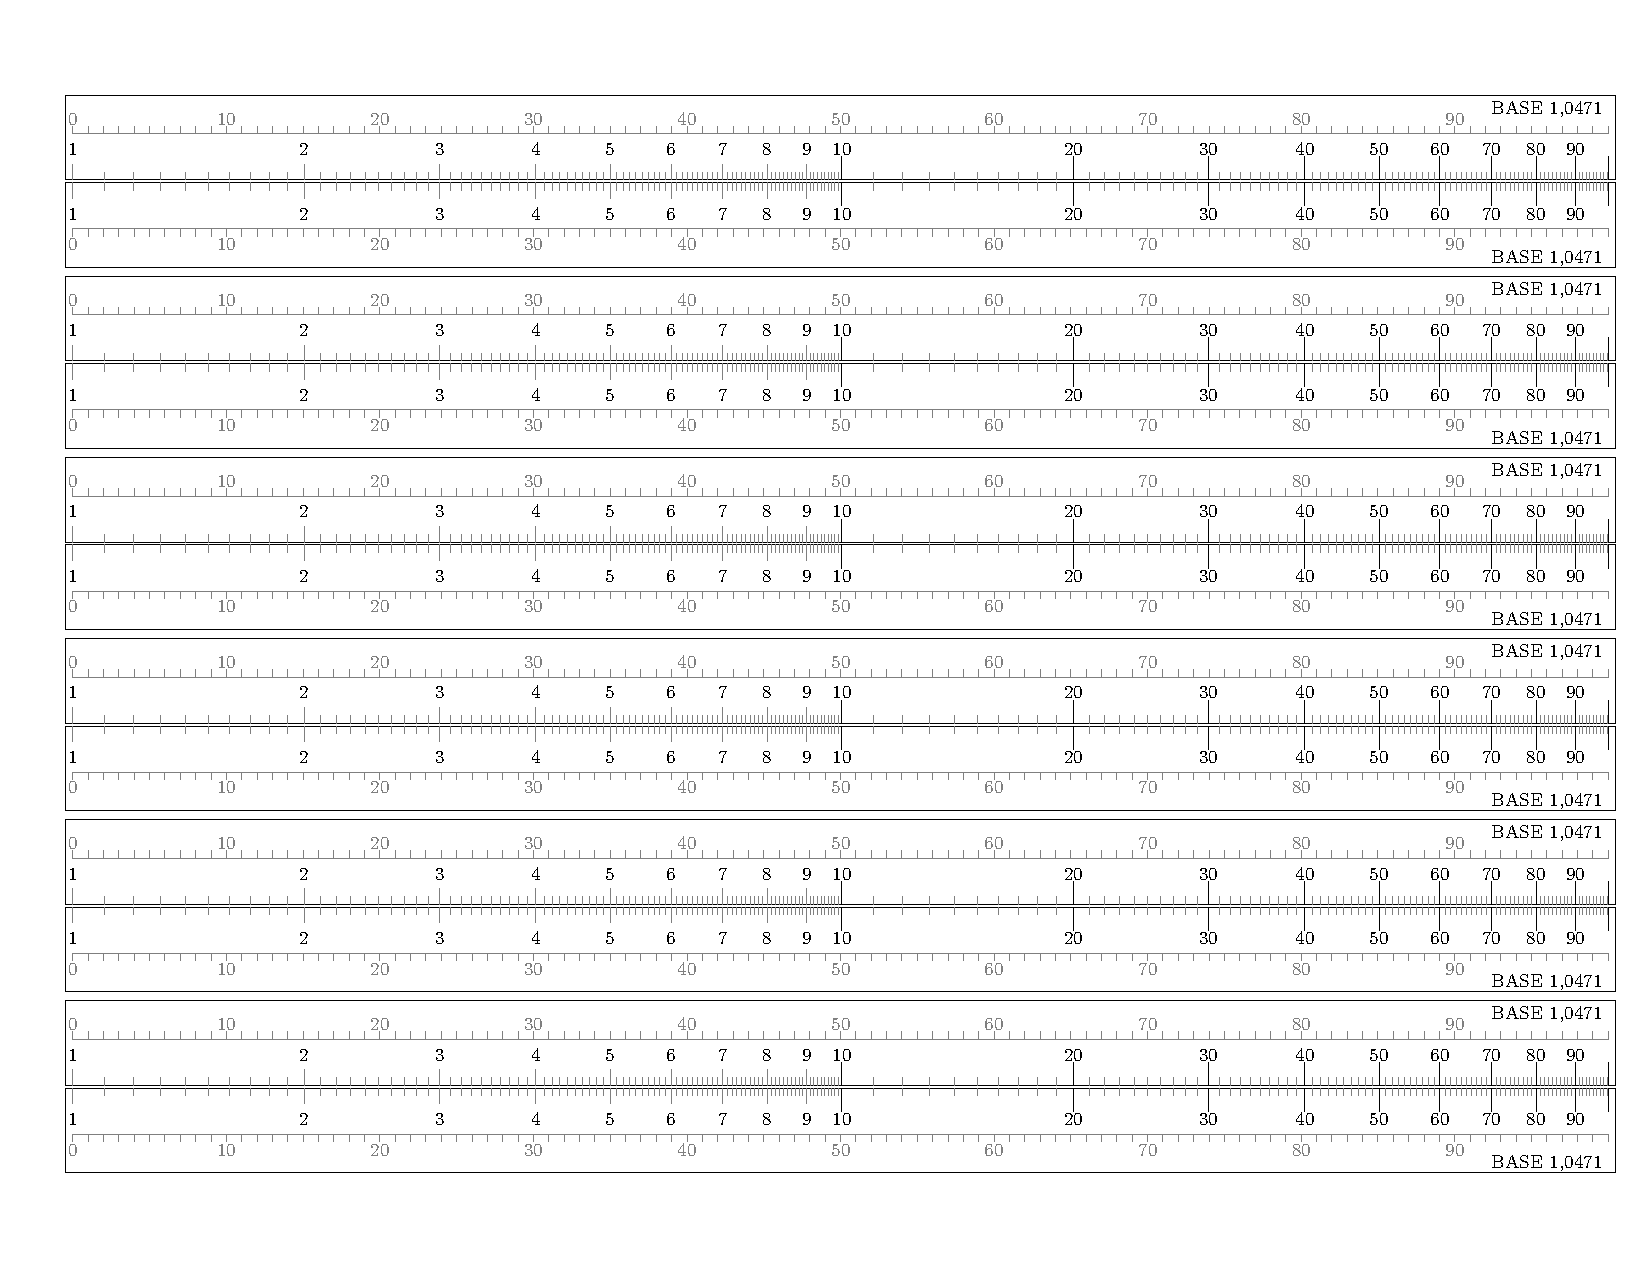
\includepdf[angle=-90]{../../../../Figuras/Ruler.pdf}
\end{center}


\end{document}